\documentclass[twoside]{book}

% Packages required by doxygen
\usepackage{fixltx2e}
\usepackage{calc}
\usepackage{doxygen}
\usepackage[export]{adjustbox} % also loads graphicx
\usepackage{graphicx}
\usepackage[utf8]{inputenc}
\usepackage{makeidx}
\usepackage{multicol}
\usepackage{multirow}
\PassOptionsToPackage{warn}{textcomp}
\usepackage{textcomp}
\usepackage[nointegrals]{wasysym}
\usepackage[table]{xcolor}

% NLS support packages
\usepackage[french]{babel}

% Font selection
\usepackage[T1]{fontenc}
\usepackage[scaled=.90]{helvet}
\usepackage{courier}
\usepackage{amssymb}
\usepackage{sectsty}
\renewcommand{\familydefault}{\sfdefault}
\allsectionsfont{%
  \fontseries{bc}\selectfont%
  \color{darkgray}%
}
\renewcommand{\DoxyLabelFont}{%
  \fontseries{bc}\selectfont%
  \color{darkgray}%
}
\newcommand{\+}{\discretionary{\mbox{\scriptsize$\hookleftarrow$}}{}{}}

% Page & text layout
\usepackage{geometry}
\geometry{%
  a4paper,%
  top=2.5cm,%
  bottom=2.5cm,%
  left=2.5cm,%
  right=2.5cm%
}
\tolerance=750
\hfuzz=15pt
\hbadness=750
\setlength{\emergencystretch}{15pt}
\setlength{\parindent}{0cm}
\setlength{\parskip}{3ex plus 2ex minus 2ex}
\makeatletter
\renewcommand{\paragraph}{%
  \@startsection{paragraph}{4}{0ex}{-1.0ex}{1.0ex}{%
    \normalfont\normalsize\bfseries\SS@parafont%
  }%
}
\renewcommand{\subparagraph}{%
  \@startsection{subparagraph}{5}{0ex}{-1.0ex}{1.0ex}{%
    \normalfont\normalsize\bfseries\SS@subparafont%
  }%
}
\makeatother

% Headers & footers
\usepackage{fancyhdr}
\pagestyle{fancyplain}
\fancyhead[LE]{\fancyplain{}{\bfseries\thepage}}
\fancyhead[CE]{\fancyplain{}{}}
\fancyhead[RE]{\fancyplain{}{\bfseries\leftmark}}
\fancyhead[LO]{\fancyplain{}{\bfseries\rightmark}}
\fancyhead[CO]{\fancyplain{}{}}
\fancyhead[RO]{\fancyplain{}{\bfseries\thepage}}
\fancyfoot[LE]{\fancyplain{}{}}
\fancyfoot[CE]{\fancyplain{}{}}
\fancyfoot[RE]{\fancyplain{}{\bfseries\scriptsize Généré par Doxygen }}
\fancyfoot[LO]{\fancyplain{}{\bfseries\scriptsize Généré par Doxygen }}
\fancyfoot[CO]{\fancyplain{}{}}
\fancyfoot[RO]{\fancyplain{}{}}
\renewcommand{\footrulewidth}{0.4pt}
\renewcommand{\chaptermark}[1]{%
  \markboth{#1}{}%
}
\renewcommand{\sectionmark}[1]{%
  \markright{\thesection\ #1}%
}

% Indices & bibliography
\usepackage{natbib}
\usepackage[titles]{tocloft}
\setcounter{tocdepth}{3}
\setcounter{secnumdepth}{5}
\makeindex

% Hyperlinks (required, but should be loaded last)
\usepackage{ifpdf}
\ifpdf
  \usepackage[pdftex,pagebackref=true]{hyperref}
\else
  \usepackage[ps2pdf,pagebackref=true]{hyperref}
\fi
\hypersetup{%
  colorlinks=true,%
  linkcolor=blue,%
  citecolor=blue,%
  unicode%
}

% Custom commands
\newcommand{\clearemptydoublepage}{%
  \newpage{\pagestyle{empty}\cleardoublepage}%
}

\usepackage{caption}
\captionsetup{labelsep=space,justification=centering,font={bf},singlelinecheck=off,skip=4pt,position=top}

%===== C O N T E N T S =====

\begin{document}

% Titlepage & ToC
\hypersetup{pageanchor=false,
             bookmarksnumbered=true,
             pdfencoding=unicode
            }
\pagenumbering{alph}
\begin{titlepage}
\vspace*{7cm}
\begin{center}%
{\Large Schmou\textquotesingle{}T\+SE }\\
\vspace*{1cm}
{\large Généré par Doxygen 1.8.13}\\
\end{center}
\end{titlepage}
\clearemptydoublepage
\pagenumbering{roman}
\tableofcontents
\clearemptydoublepage
\pagenumbering{arabic}
\hypersetup{pageanchor=true}

%--- Begin generated contents ---
\chapter{Index des classes}
\section{Liste des classes}
Liste des classes, structures, unions et interfaces avec une brève description \+:\begin{DoxyCompactList}
\item\contentsline{section}{\hyperlink{class_attaque}{Attaque} }{\pageref{class_attaque}}{}
\item\contentsline{section}{\hyperlink{struct_input__base_1_1movement__input__t_1_1joypad__t_1_1joypad__input__t_1_1buttons__t}{Input\+\_\+base$<$ N $>$\+::movement\+\_\+input\+\_\+t\+::joypad\+\_\+t\+::joypad\+\_\+input\+\_\+t\+::buttons\+\_\+t} }{\pageref{struct_input__base_1_1movement__input__t_1_1joypad__t_1_1joypad__input__t_1_1buttons__t}}{}
\item\contentsline{section}{\hyperlink{class_capacite}{Capacite} \\*Classe abstraite qui définit la structure générale d\textquotesingle{}une capacité, à faire hériter de chaque capacité }{\pageref{class_capacite}}{}
\item\contentsline{section}{\hyperlink{class_cap_dash}{Cap\+Dash} }{\pageref{class_cap_dash}}{}
\item\contentsline{section}{\hyperlink{class_cap_piou}{Cap\+Piou} }{\pageref{class_cap_piou}}{}
\item\contentsline{section}{\hyperlink{class_cap_test}{Cap\+Test} }{\pageref{class_cap_test}}{}
\item\contentsline{section}{\hyperlink{class_entite}{Entite} \\*Classe virtuelle qui définit une entité }{\pageref{class_entite}}{}
\item\contentsline{section}{\hyperlink{class_input__base}{Input\+\_\+base$<$ N $>$} }{\pageref{class_input__base}}{}
\item\contentsline{section}{\hyperlink{union_input__base_1_1movement__input__t_1_1joypad__t_1_1joypad__input__t}{Input\+\_\+base$<$ N $>$\+::movement\+\_\+input\+\_\+t\+::joypad\+\_\+t\+::joypad\+\_\+input\+\_\+t} }{\pageref{union_input__base_1_1movement__input__t_1_1joypad__t_1_1joypad__input__t}}{}
\item\contentsline{section}{\hyperlink{struct_input__base_1_1movement__input__t_1_1joypad__t}{Input\+\_\+base$<$ N $>$\+::movement\+\_\+input\+\_\+t\+::joypad\+\_\+t} }{\pageref{struct_input__base_1_1movement__input__t_1_1joypad__t}}{}
\item\contentsline{section}{\hyperlink{struct_input__base_1_1movement__input__t_1_1joypad__t_1_1joypad__input__t_1_1joysticks__t}{Input\+\_\+base$<$ N $>$\+::movement\+\_\+input\+\_\+t\+::joypad\+\_\+t\+::joypad\+\_\+input\+\_\+t\+::joysticks\+\_\+t} }{\pageref{struct_input__base_1_1movement__input__t_1_1joypad__t_1_1joypad__input__t_1_1joysticks__t}}{}
\item\contentsline{section}{\hyperlink{struct_input__base_1_1movement__input__t_1_1keyboard__t}{Input\+\_\+base$<$ N $>$\+::movement\+\_\+input\+\_\+t\+::keyboard\+\_\+t} }{\pageref{struct_input__base_1_1movement__input__t_1_1keyboard__t}}{}
\item\contentsline{section}{\hyperlink{struct_input__base_1_1movement__input__t_1_1mouse__t}{Input\+\_\+base$<$ N $>$\+::movement\+\_\+input\+\_\+t\+::mouse\+\_\+t} }{\pageref{struct_input__base_1_1movement__input__t_1_1mouse__t}}{}
\item\contentsline{section}{\hyperlink{class_partie}{Partie} \\*Description brève }{\pageref{class_partie}}{}
\item\contentsline{section}{\hyperlink{class_projectile}{Projectile} \\*Classe abstraite qui définit la structure générale d\textquotesingle{}un projectile, à faire hériter pour chaque projectile }{\pageref{class_projectile}}{}
\item\contentsline{section}{\hyperlink{class_projectile_piou_piou}{Projectile\+Piou\+Piou} }{\pageref{class_projectile_piou_piou}}{}
\item\contentsline{section}{\hyperlink{class_proj_piou}{Proj\+Piou} }{\pageref{class_proj_piou}}{}
\item\contentsline{section}{\hyperlink{class_proj_test}{Proj\+Test} }{\pageref{class_proj_test}}{}
\item\contentsline{section}{\hyperlink{class_vaisseau}{Vaisseau} \\*Classe du vaisseau (véhicule) d\textquotesingle{}un joueur ou d\textquotesingle{}un ennemi }{\pageref{class_vaisseau}}{}
\item\contentsline{section}{\hyperlink{class_vaisseau_test}{Vaisseau\+Test} }{\pageref{class_vaisseau_test}}{}
\end{DoxyCompactList}

\chapter{Index des fichiers}
\section{Liste des fichiers}
Liste de tous les fichiers avec une brève description \+:\begin{DoxyCompactList}
\item\contentsline{section}{src/\hyperlink{constantes_8h}{constantes.\+h} }{\pageref{constantes_8h}}{}
\item\contentsline{section}{src/\hyperlink{_entite_8cpp}{Entite.\+cpp} }{\pageref{_entite_8cpp}}{}
\item\contentsline{section}{src/\hyperlink{_entite_8h}{Entite.\+h} }{\pageref{_entite_8h}}{}
\item\contentsline{section}{src/\hyperlink{main_8cpp}{main.\+cpp} }{\pageref{main_8cpp}}{}
\item\contentsline{section}{src/\hyperlink{_partie_8cpp}{Partie.\+cpp} }{\pageref{_partie_8cpp}}{}
\item\contentsline{section}{src/\hyperlink{_partie_8h}{Partie.\+h} }{\pageref{_partie_8h}}{}
\item\contentsline{section}{src/\+Capacites/\hyperlink{___capacites_8h}{\+\_\+\+Capacites.\+h} }{\pageref{___capacites_8h}}{}
\item\contentsline{section}{src/\+Capacites/\hyperlink{_capacite_8cpp}{Capacite.\+cpp} }{\pageref{_capacite_8cpp}}{}
\item\contentsline{section}{src/\+Capacites/\hyperlink{_capacite_8h}{Capacite.\+h} }{\pageref{_capacite_8h}}{}
\item\contentsline{section}{src/\+Capacites/\hyperlink{_cap_dash_8cpp}{Cap\+Dash.\+cpp} }{\pageref{_cap_dash_8cpp}}{}
\item\contentsline{section}{src/\+Capacites/\hyperlink{_cap_dash_8h}{Cap\+Dash.\+h} }{\pageref{_cap_dash_8h}}{}
\item\contentsline{section}{src/\+Capacites/\hyperlink{_cap_piou_8cpp}{Cap\+Piou.\+cpp} }{\pageref{_cap_piou_8cpp}}{}
\item\contentsline{section}{src/\+Capacites/\hyperlink{_cap_piou_8h}{Cap\+Piou.\+h} }{\pageref{_cap_piou_8h}}{}
\item\contentsline{section}{src/\+Capacites/\hyperlink{_cap_test_8cpp}{Cap\+Test.\+cpp} }{\pageref{_cap_test_8cpp}}{}
\item\contentsline{section}{src/\+Capacites/\hyperlink{_cap_test_8h}{Cap\+Test.\+h} }{\pageref{_cap_test_8h}}{}
\item\contentsline{section}{src/\+Interface/\hyperlink{_input_8cpp}{Input.\+cpp} }{\pageref{_input_8cpp}}{}
\item\contentsline{section}{src/\+Interface/\hyperlink{_input_8h}{Input.\+h} }{\pageref{_input_8h}}{}
\item\contentsline{section}{src/\+Projectiles/\hyperlink{__projectiles_8h}{\+\_\+projectiles.\+h} }{\pageref{__projectiles_8h}}{}
\item\contentsline{section}{src/\+Projectiles/\hyperlink{_projectile_8cpp}{Projectile.\+cpp} }{\pageref{_projectile_8cpp}}{}
\item\contentsline{section}{src/\+Projectiles/\hyperlink{_projectile_8h}{Projectile.\+h} }{\pageref{_projectile_8h}}{}
\item\contentsline{section}{src/\+Projectiles/\hyperlink{_proj_piou_8cpp}{Proj\+Piou.\+cpp} }{\pageref{_proj_piou_8cpp}}{}
\item\contentsline{section}{src/\+Projectiles/\hyperlink{_proj_piou_8h}{Proj\+Piou.\+h} }{\pageref{_proj_piou_8h}}{}
\item\contentsline{section}{src/\+Projectiles/\hyperlink{_proj_test_8cpp}{Proj\+Test.\+cpp} }{\pageref{_proj_test_8cpp}}{}
\item\contentsline{section}{src/\+Projectiles/\hyperlink{_proj_test_8h}{Proj\+Test.\+h} }{\pageref{_proj_test_8h}}{}
\item\contentsline{section}{src/\+Utilitaires/\hyperlink{_collision_8cpp}{Collision.\+cpp} }{\pageref{_collision_8cpp}}{}
\item\contentsline{section}{src/\+Utilitaires/\hyperlink{_collision_8h}{Collision.\+h} }{\pageref{_collision_8h}}{}
\item\contentsline{section}{src/\+Vaisseau/\hyperlink{__vaisseaux_8h}{\+\_\+vaisseaux.\+h} }{\pageref{__vaisseaux_8h}}{}
\item\contentsline{section}{src/\+Vaisseau/\hyperlink{_vaisseau_8cpp}{Vaisseau.\+cpp} }{\pageref{_vaisseau_8cpp}}{}
\item\contentsline{section}{src/\+Vaisseau/\hyperlink{_vaisseau_8h}{Vaisseau.\+h} }{\pageref{_vaisseau_8h}}{}
\item\contentsline{section}{src/\+Vaisseau/\hyperlink{_vaisseau_eclaireur_8cpp}{Vaisseau\+Eclaireur.\+cpp} }{\pageref{_vaisseau_eclaireur_8cpp}}{}
\item\contentsline{section}{src/\+Vaisseau/\hyperlink{_vaisseau_eclaireur_8h}{Vaisseau\+Eclaireur.\+h} }{\pageref{_vaisseau_eclaireur_8h}}{}
\item\contentsline{section}{src/\+Vaisseau/\hyperlink{_vaisseau_test_8cpp}{Vaisseau\+Test.\+cpp} }{\pageref{_vaisseau_test_8cpp}}{}
\item\contentsline{section}{src/\+Vaisseau/\hyperlink{_vaisseau_test_8h}{Vaisseau\+Test.\+h} }{\pageref{_vaisseau_test_8h}}{}
\end{DoxyCompactList}

\chapter{Documentation des classes}
\hypertarget{class_capacite}{}\section{Référence de la classe Capacite}
\label{class_capacite}\index{Capacite@{Capacite}}


Classe abstraite qui définit la structure générale d\textquotesingle{}une capacité, à faire hériter de chaque capacité  




{\ttfamily \#include $<$Capacite.\+h$>$}



Graphe d\textquotesingle{}héritage de Capacite\+:\nopagebreak
\begin{figure}[H]
\begin{center}
\leavevmode
\includegraphics[width=282pt]{class_capacite__inherit__graph}
\end{center}
\end{figure}
\subsection*{Fonctions membres publiques}
\begin{DoxyCompactItemize}
\item 
\hyperlink{class_capacite_a8a1aebc5b2332e366a3f207c23b4d363}{Capacite} ()=default
\item 
virtual \hyperlink{class_capacite_a687ff139afef118ebb63b897861674fd}{$\sim$\+Capacite} ()=default
\item 
int const \hyperlink{class_capacite_a1842888fc39a0054d3cc9d7236ab1191}{get\+Cooldown} ()
\item 
int const \hyperlink{class_capacite_a82e4eebf522c02163725872b288bfcf8}{get\+Time} ()
\item 
std\+::string const \hyperlink{class_capacite_a96218b289768ff461ffaaa0abe014a42}{get\+Nom} ()
\item 
virtual void \hyperlink{class_capacite_a4d4f643987fcc2168567bf28a36ea418}{utiliser} (int x, int y)=0
\item 
virtual void \hyperlink{class_capacite_a7d4e86c20cd198960f25c0eb443148fe}{actualiser} (std\+::vector$<$ \hyperlink{class_projectile}{Projectile} $\ast$$>$ \&projectiles, \hyperlink{class_entite}{Entite} $\ast$vaisseau)=0
\end{DoxyCompactItemize}
\subsection*{Attributs protégés}
\begin{DoxyCompactItemize}
\item 
int \hyperlink{class_capacite_abc3eb04129009107c0b60b03e7a3ff06}{debut\+X\+\_\+}
\item 
int \hyperlink{class_capacite_a741d48934a015c226b15e6519724e400}{debut\+Y\+\_\+}
\item 
int \hyperlink{class_capacite_aabb946971871ffbcb9bb9a4d9cd3c0c3}{cooldown\+\_\+}
\item 
int \hyperlink{class_capacite_ac743cb7c9605c9e3205885cdcf14d2dd}{t\+\_\+}
\item 
std\+::string \hyperlink{class_capacite_a430472b509233086cbad1d6d8332dc8c}{nom\+\_\+}
\end{DoxyCompactItemize}


\subsection{Description détaillée}
Classe abstraite qui définit la structure générale d\textquotesingle{}une capacité, à faire hériter de chaque capacité 

Cette classe abstraite permet de définir la structure générale d\textquotesingle{}une capacité du jeu, elle doit être héritée pour chaque capacité qui est ajoutée au jeu 

\subsection{Documentation des constructeurs et destructeur}
\mbox{\Hypertarget{class_capacite_a8a1aebc5b2332e366a3f207c23b4d363}\label{class_capacite_a8a1aebc5b2332e366a3f207c23b4d363}} 
\index{Capacite@{Capacite}!Capacite@{Capacite}}
\index{Capacite@{Capacite}!Capacite@{Capacite}}
\subsubsection{\texorpdfstring{Capacite()}{Capacite()}}
{\footnotesize\ttfamily Capacite\+::\+Capacite (\begin{DoxyParamCaption}{ }\end{DoxyParamCaption})\hspace{0.3cm}{\ttfamily [default]}}

\mbox{\Hypertarget{class_capacite_a687ff139afef118ebb63b897861674fd}\label{class_capacite_a687ff139afef118ebb63b897861674fd}} 
\index{Capacite@{Capacite}!````~Capacite@{$\sim$\+Capacite}}
\index{````~Capacite@{$\sim$\+Capacite}!Capacite@{Capacite}}
\subsubsection{\texorpdfstring{$\sim$\+Capacite()}{~Capacite()}}
{\footnotesize\ttfamily virtual Capacite\+::$\sim$\+Capacite (\begin{DoxyParamCaption}{ }\end{DoxyParamCaption})\hspace{0.3cm}{\ttfamily [virtual]}, {\ttfamily [default]}}



\subsection{Documentation des fonctions membres}
\mbox{\Hypertarget{class_capacite_a7d4e86c20cd198960f25c0eb443148fe}\label{class_capacite_a7d4e86c20cd198960f25c0eb443148fe}} 
\index{Capacite@{Capacite}!actualiser@{actualiser}}
\index{actualiser@{actualiser}!Capacite@{Capacite}}
\subsubsection{\texorpdfstring{actualiser()}{actualiser()}}
{\footnotesize\ttfamily virtual void Capacite\+::actualiser (\begin{DoxyParamCaption}\item[{std\+::vector$<$ \hyperlink{class_projectile}{Projectile} $\ast$$>$ \&}]{projectiles,  }\item[{\hyperlink{class_entite}{Entite} $\ast$}]{vaisseau }\end{DoxyParamCaption})\hspace{0.3cm}{\ttfamily [pure virtual]}}



Implémenté dans \hyperlink{class_cap_dash_a886522c648db49b81c330737ad96a517}{Cap\+Dash}, \hyperlink{class_cap_piou_aabdcaa253f10db2bca12e750005485fc}{Cap\+Piou}, et \hyperlink{class_cap_test_a5742770894ff765e2785f82aab88b223}{Cap\+Test}.

\mbox{\Hypertarget{class_capacite_a1842888fc39a0054d3cc9d7236ab1191}\label{class_capacite_a1842888fc39a0054d3cc9d7236ab1191}} 
\index{Capacite@{Capacite}!get\+Cooldown@{get\+Cooldown}}
\index{get\+Cooldown@{get\+Cooldown}!Capacite@{Capacite}}
\subsubsection{\texorpdfstring{get\+Cooldown()}{getCooldown()}}
{\footnotesize\ttfamily int const Capacite\+::get\+Cooldown (\begin{DoxyParamCaption}{ }\end{DoxyParamCaption})\hspace{0.3cm}{\ttfamily [inline]}}

\mbox{\Hypertarget{class_capacite_a96218b289768ff461ffaaa0abe014a42}\label{class_capacite_a96218b289768ff461ffaaa0abe014a42}} 
\index{Capacite@{Capacite}!get\+Nom@{get\+Nom}}
\index{get\+Nom@{get\+Nom}!Capacite@{Capacite}}
\subsubsection{\texorpdfstring{get\+Nom()}{getNom()}}
{\footnotesize\ttfamily std\+::string const Capacite\+::get\+Nom (\begin{DoxyParamCaption}{ }\end{DoxyParamCaption})\hspace{0.3cm}{\ttfamily [inline]}}

\mbox{\Hypertarget{class_capacite_a82e4eebf522c02163725872b288bfcf8}\label{class_capacite_a82e4eebf522c02163725872b288bfcf8}} 
\index{Capacite@{Capacite}!get\+Time@{get\+Time}}
\index{get\+Time@{get\+Time}!Capacite@{Capacite}}
\subsubsection{\texorpdfstring{get\+Time()}{getTime()}}
{\footnotesize\ttfamily int const Capacite\+::get\+Time (\begin{DoxyParamCaption}{ }\end{DoxyParamCaption})\hspace{0.3cm}{\ttfamily [inline]}}

\mbox{\Hypertarget{class_capacite_a4d4f643987fcc2168567bf28a36ea418}\label{class_capacite_a4d4f643987fcc2168567bf28a36ea418}} 
\index{Capacite@{Capacite}!utiliser@{utiliser}}
\index{utiliser@{utiliser}!Capacite@{Capacite}}
\subsubsection{\texorpdfstring{utiliser()}{utiliser()}}
{\footnotesize\ttfamily virtual void Capacite\+::utiliser (\begin{DoxyParamCaption}\item[{int}]{x,  }\item[{int}]{y }\end{DoxyParamCaption})\hspace{0.3cm}{\ttfamily [pure virtual]}}



Implémenté dans \hyperlink{class_cap_dash_ada59ecb62d2c18f6bb6b4acf28a2da93}{Cap\+Dash}, \hyperlink{class_cap_piou_a20ed7a993ce209a3df246f655f107f22}{Cap\+Piou}, et \hyperlink{class_cap_test_af85984f6d9330e5527feff1a62ee4242}{Cap\+Test}.



\subsection{Documentation des données membres}
\mbox{\Hypertarget{class_capacite_aabb946971871ffbcb9bb9a4d9cd3c0c3}\label{class_capacite_aabb946971871ffbcb9bb9a4d9cd3c0c3}} 
\index{Capacite@{Capacite}!cooldown\+\_\+@{cooldown\+\_\+}}
\index{cooldown\+\_\+@{cooldown\+\_\+}!Capacite@{Capacite}}
\subsubsection{\texorpdfstring{cooldown\+\_\+}{cooldown\_}}
{\footnotesize\ttfamily int Capacite\+::cooldown\+\_\+\hspace{0.3cm}{\ttfamily [protected]}}

\mbox{\Hypertarget{class_capacite_abc3eb04129009107c0b60b03e7a3ff06}\label{class_capacite_abc3eb04129009107c0b60b03e7a3ff06}} 
\index{Capacite@{Capacite}!debut\+X\+\_\+@{debut\+X\+\_\+}}
\index{debut\+X\+\_\+@{debut\+X\+\_\+}!Capacite@{Capacite}}
\subsubsection{\texorpdfstring{debut\+X\+\_\+}{debutX\_}}
{\footnotesize\ttfamily int Capacite\+::debut\+X\+\_\+\hspace{0.3cm}{\ttfamily [protected]}}

\mbox{\Hypertarget{class_capacite_a741d48934a015c226b15e6519724e400}\label{class_capacite_a741d48934a015c226b15e6519724e400}} 
\index{Capacite@{Capacite}!debut\+Y\+\_\+@{debut\+Y\+\_\+}}
\index{debut\+Y\+\_\+@{debut\+Y\+\_\+}!Capacite@{Capacite}}
\subsubsection{\texorpdfstring{debut\+Y\+\_\+}{debutY\_}}
{\footnotesize\ttfamily int Capacite\+::debut\+Y\+\_\+\hspace{0.3cm}{\ttfamily [protected]}}

\mbox{\Hypertarget{class_capacite_a430472b509233086cbad1d6d8332dc8c}\label{class_capacite_a430472b509233086cbad1d6d8332dc8c}} 
\index{Capacite@{Capacite}!nom\+\_\+@{nom\+\_\+}}
\index{nom\+\_\+@{nom\+\_\+}!Capacite@{Capacite}}
\subsubsection{\texorpdfstring{nom\+\_\+}{nom\_}}
{\footnotesize\ttfamily std\+::string Capacite\+::nom\+\_\+\hspace{0.3cm}{\ttfamily [protected]}}

\mbox{\Hypertarget{class_capacite_ac743cb7c9605c9e3205885cdcf14d2dd}\label{class_capacite_ac743cb7c9605c9e3205885cdcf14d2dd}} 
\index{Capacite@{Capacite}!t\+\_\+@{t\+\_\+}}
\index{t\+\_\+@{t\+\_\+}!Capacite@{Capacite}}
\subsubsection{\texorpdfstring{t\+\_\+}{t\_}}
{\footnotesize\ttfamily int Capacite\+::t\+\_\+\hspace{0.3cm}{\ttfamily [protected]}}



La documentation de cette classe a été générée à partir du fichier suivant \+:\begin{DoxyCompactItemize}
\item 
src/\hyperlink{_capacite_8h}{Capacite.\+h}\end{DoxyCompactItemize}

\hypertarget{class_partie}{}\section{Référence de la classe Partie}
\label{class_partie}\index{Partie@{Partie}}


Description brève.  




{\ttfamily \#include $<$Partie.\+h$>$}

\subsection*{Fonctions membres publiques}
\begin{DoxyCompactItemize}
\item 
\hyperlink{class_partie_ae40831aad10fc4a391295e2ea1447b5a}{Partie} ()
\item 
\hyperlink{class_partie_ae4afeb7336bb84427272cfb7018b5e3d}{$\sim$\+Partie} ()
\end{DoxyCompactItemize}


\subsection{Description détaillée}
Description brève. 

Description détaillée 

\subsection{Documentation des constructeurs et destructeur}
\mbox{\Hypertarget{class_partie_ae40831aad10fc4a391295e2ea1447b5a}\label{class_partie_ae40831aad10fc4a391295e2ea1447b5a}} 
\index{Partie@{Partie}!Partie@{Partie}}
\index{Partie@{Partie}!Partie@{Partie}}
\subsubsection{\texorpdfstring{Partie()}{Partie()}}
{\footnotesize\ttfamily Partie\+::\+Partie (\begin{DoxyParamCaption}{ }\end{DoxyParamCaption})}

\mbox{\Hypertarget{class_partie_ae4afeb7336bb84427272cfb7018b5e3d}\label{class_partie_ae4afeb7336bb84427272cfb7018b5e3d}} 
\index{Partie@{Partie}!````~Partie@{$\sim$\+Partie}}
\index{````~Partie@{$\sim$\+Partie}!Partie@{Partie}}
\subsubsection{\texorpdfstring{$\sim$\+Partie()}{~Partie()}}
{\footnotesize\ttfamily Partie\+::$\sim$\+Partie (\begin{DoxyParamCaption}{ }\end{DoxyParamCaption})}



La documentation de cette classe a été générée à partir du fichier suivant \+:\begin{DoxyCompactItemize}
\item 
src/\hyperlink{_partie_8h}{Partie.\+h}\end{DoxyCompactItemize}

\hypertarget{class_projectile}{}\section{Référence de la classe Projectile}
\label{class_projectile}\index{Projectile@{Projectile}}


Classe abstraite qui définit la structure générale d\textquotesingle{}un projectile, à faire hériter pour chaque projectile.  




{\ttfamily \#include $<$Projectile.\+h$>$}



Graphe d\textquotesingle{}héritage de Projectile\+:
\nopagebreak
\begin{figure}[H]
\begin{center}
\leavevmode
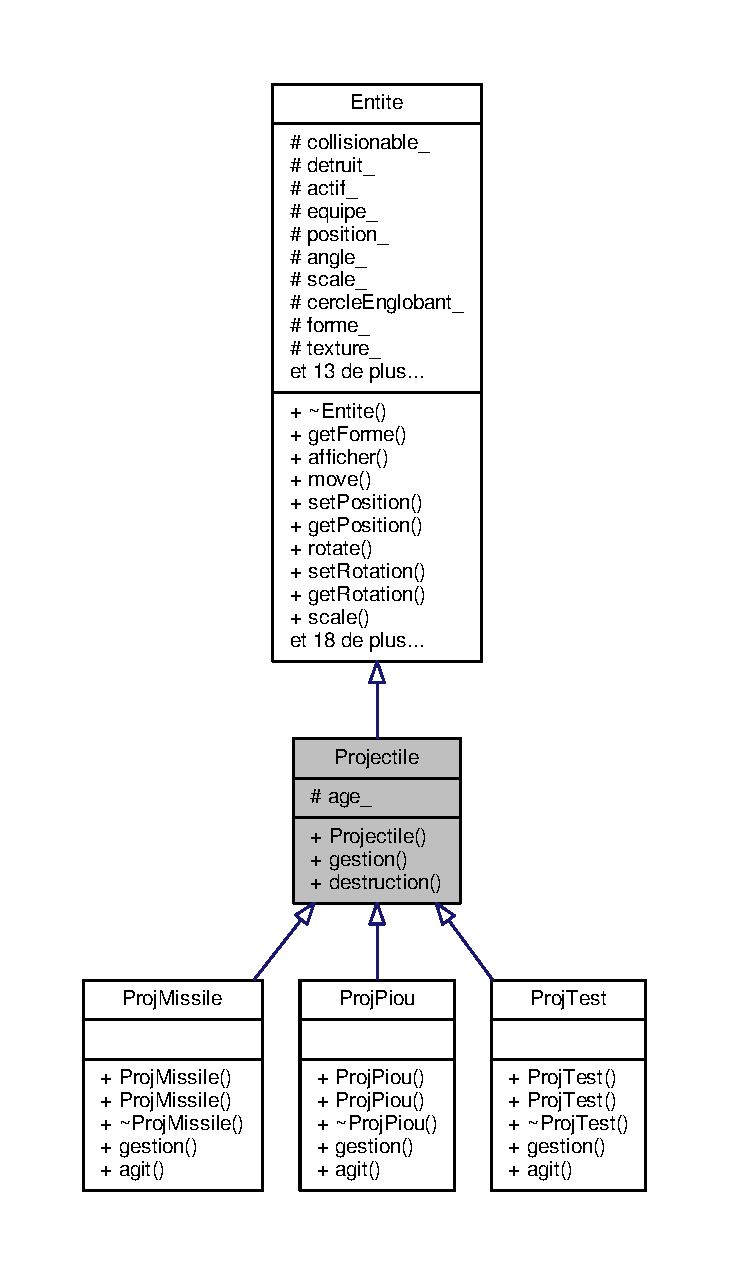
\includegraphics[width=204pt]{class_projectile__inherit__graph}
\end{center}
\end{figure}


Graphe de collaboration de Projectile\+:\nopagebreak
\begin{figure}[H]
\begin{center}
\leavevmode
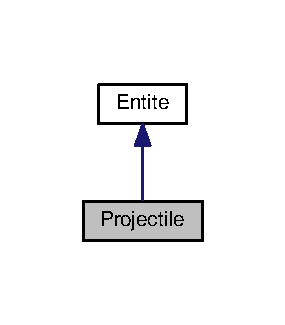
\includegraphics[width=137pt]{class_projectile__coll__graph}
\end{center}
\end{figure}
\subsection*{Fonctions membres publiques}
\begin{DoxyCompactItemize}
\item 
\hyperlink{class_projectile_ac536ed2aad56af866a2078b9a85aa16d}{Projectile} ()
\item 
virtual void \hyperlink{class_projectile_aa969857f9837d9be3a6ea415c9ba3ff1}{gestion} (sf\+::\+Render\+Window \&window)=0
\end{DoxyCompactItemize}
\subsection*{Attributs protégés}
\begin{DoxyCompactItemize}
\item 
int \hyperlink{class_projectile_a1f0a231e002d4796c32ccfeb36c887b1}{age\+\_\+}
\end{DoxyCompactItemize}


\subsection{Description détaillée}
Classe abstraite qui définit la structure générale d\textquotesingle{}un projectile, à faire hériter pour chaque projectile. 

Classe abstraite mère de chaque projectile en tant qu\textquotesingle{}entité propre. Une capacité peut créer plusieurs projectiles ; elle leur donne des méthodes qui les font exister dans la boucle de jeu \+: déplacement, test de collison, dégats... 

\subsection{Documentation des constructeurs et destructeur}
\mbox{\Hypertarget{class_projectile_ac536ed2aad56af866a2078b9a85aa16d}\label{class_projectile_ac536ed2aad56af866a2078b9a85aa16d}} 
\index{Projectile@{Projectile}!Projectile@{Projectile}}
\index{Projectile@{Projectile}!Projectile@{Projectile}}
\subsubsection{\texorpdfstring{Projectile()}{Projectile()}}
{\footnotesize\ttfamily Projectile\+::\+Projectile (\begin{DoxyParamCaption}{ }\end{DoxyParamCaption})}



\subsection{Documentation des fonctions membres}
\mbox{\Hypertarget{class_projectile_aa969857f9837d9be3a6ea415c9ba3ff1}\label{class_projectile_aa969857f9837d9be3a6ea415c9ba3ff1}} 
\index{Projectile@{Projectile}!gestion@{gestion}}
\index{gestion@{gestion}!Projectile@{Projectile}}
\subsubsection{\texorpdfstring{gestion()}{gestion()}}
{\footnotesize\ttfamily virtual void Projectile\+::gestion (\begin{DoxyParamCaption}\item[{sf\+::\+Render\+Window \&}]{window }\end{DoxyParamCaption})\hspace{0.3cm}{\ttfamily [pure virtual]}}



Implémenté dans \hyperlink{class_proj_test_af0b751a8e8cb0b7d10857722b691f3b6}{Proj\+Test}, et \hyperlink{class_proj_piou_a964182d333ed2bf64408a7812bc4cd28}{Proj\+Piou}.



\subsection{Documentation des données membres}
\mbox{\Hypertarget{class_projectile_a1f0a231e002d4796c32ccfeb36c887b1}\label{class_projectile_a1f0a231e002d4796c32ccfeb36c887b1}} 
\index{Projectile@{Projectile}!age\+\_\+@{age\+\_\+}}
\index{age\+\_\+@{age\+\_\+}!Projectile@{Projectile}}
\subsubsection{\texorpdfstring{age\+\_\+}{age\_}}
{\footnotesize\ttfamily int Projectile\+::age\+\_\+\hspace{0.3cm}{\ttfamily [protected]}}



La documentation de cette classe a été générée à partir des fichiers suivants \+:\begin{DoxyCompactItemize}
\item 
src/\+Projectiles/\hyperlink{_projectile_8h}{Projectile.\+h}\item 
src/\+Projectiles/\hyperlink{_projectile_8cpp}{Projectile.\+cpp}\end{DoxyCompactItemize}

\hypertarget{class_vaisseau}{}\section{Référence de la classe Vaisseau}
\label{class_vaisseau}\index{Vaisseau@{Vaisseau}}


classe du vaisseau (véhicule) d\textquotesingle{}un joueur ou d\textquotesingle{}un ennemi  




{\ttfamily \#include $<$Vaisseau.\+h$>$}

\subsection*{Fonctions membres publiques}
\begin{DoxyCompactItemize}
\item 
\hyperlink{class_vaisseau_a7a6f829d62d9a0568c0c10d42c81bd47}{Vaisseau} (bool player)
\item 
\hyperlink{class_vaisseau_ae40b8e0143d6b736065207281bde2e8a}{$\sim$\+Vaisseau} ()
\end{DoxyCompactItemize}


\subsection{Description détaillée}
classe du vaisseau (véhicule) d\textquotesingle{}un joueur ou d\textquotesingle{}un ennemi 

Description détaillée 

\subsection{Documentation des constructeurs et destructeur}
\mbox{\Hypertarget{class_vaisseau_a7a6f829d62d9a0568c0c10d42c81bd47}\label{class_vaisseau_a7a6f829d62d9a0568c0c10d42c81bd47}} 
\index{Vaisseau@{Vaisseau}!Vaisseau@{Vaisseau}}
\index{Vaisseau@{Vaisseau}!Vaisseau@{Vaisseau}}
\subsubsection{\texorpdfstring{Vaisseau()}{Vaisseau()}}
{\footnotesize\ttfamily Vaisseau\+::\+Vaisseau (\begin{DoxyParamCaption}\item[{bool}]{player }\end{DoxyParamCaption})\hspace{0.3cm}{\ttfamily [explicit]}}

\mbox{\Hypertarget{class_vaisseau_ae40b8e0143d6b736065207281bde2e8a}\label{class_vaisseau_ae40b8e0143d6b736065207281bde2e8a}} 
\index{Vaisseau@{Vaisseau}!````~Vaisseau@{$\sim$\+Vaisseau}}
\index{````~Vaisseau@{$\sim$\+Vaisseau}!Vaisseau@{Vaisseau}}
\subsubsection{\texorpdfstring{$\sim$\+Vaisseau()}{~Vaisseau()}}
{\footnotesize\ttfamily Vaisseau\+::$\sim$\+Vaisseau (\begin{DoxyParamCaption}{ }\end{DoxyParamCaption})}



La documentation de cette classe a été générée à partir des fichiers suivants \+:\begin{DoxyCompactItemize}
\item 
src/\hyperlink{_vaisseau_8h}{Vaisseau.\+h}\item 
src/\hyperlink{_vaisseau_8cpp}{Vaisseau.\+cpp}\end{DoxyCompactItemize}

\chapter{Documentation des fichiers}
\hypertarget{_capacite_8h}{}\section{Référence du fichier src/\+Capacite.h}
\label{_capacite_8h}\index{src/\+Capacite.\+h@{src/\+Capacite.\+h}}
\subsection*{Classes}
\begin{DoxyCompactItemize}
\item 
class \hyperlink{class_capacite}{Capacite}
\begin{DoxyCompactList}\small\item\em Classe virtuelle qui définit la structure générale d\textquotesingle{}une capacité \end{DoxyCompactList}\end{DoxyCompactItemize}

\hypertarget{main_8cpp}{}\section{Référence du fichier src/main.cpp}
\label{main_8cpp}\index{src/main.\+cpp@{src/main.\+cpp}}
{\ttfamily \#include $<$S\+F\+M\+L/\+Graphics.\+hpp$>$}\newline
{\ttfamily \#include $<$cmath$>$}\newline
{\ttfamily \#include $<$ctime$>$}\newline
{\ttfamily \#include $<$iostream$>$}\newline
{\ttfamily \#include \char`\"{}constantes.\+h\char`\"{}}\newline
{\ttfamily \#include \char`\"{}Entite.\+h\char`\"{}}\newline
{\ttfamily \#include \char`\"{}Collision.\+h\char`\"{}}\newline
{\ttfamily \#include \char`\"{}Partie.\+h\char`\"{}}\newline
{\ttfamily \#include \char`\"{}Input.\+h\char`\"{}}\newline
Graphe des dépendances par inclusion de main.\+cpp\+:
\nopagebreak
\begin{figure}[H]
\begin{center}
\leavevmode
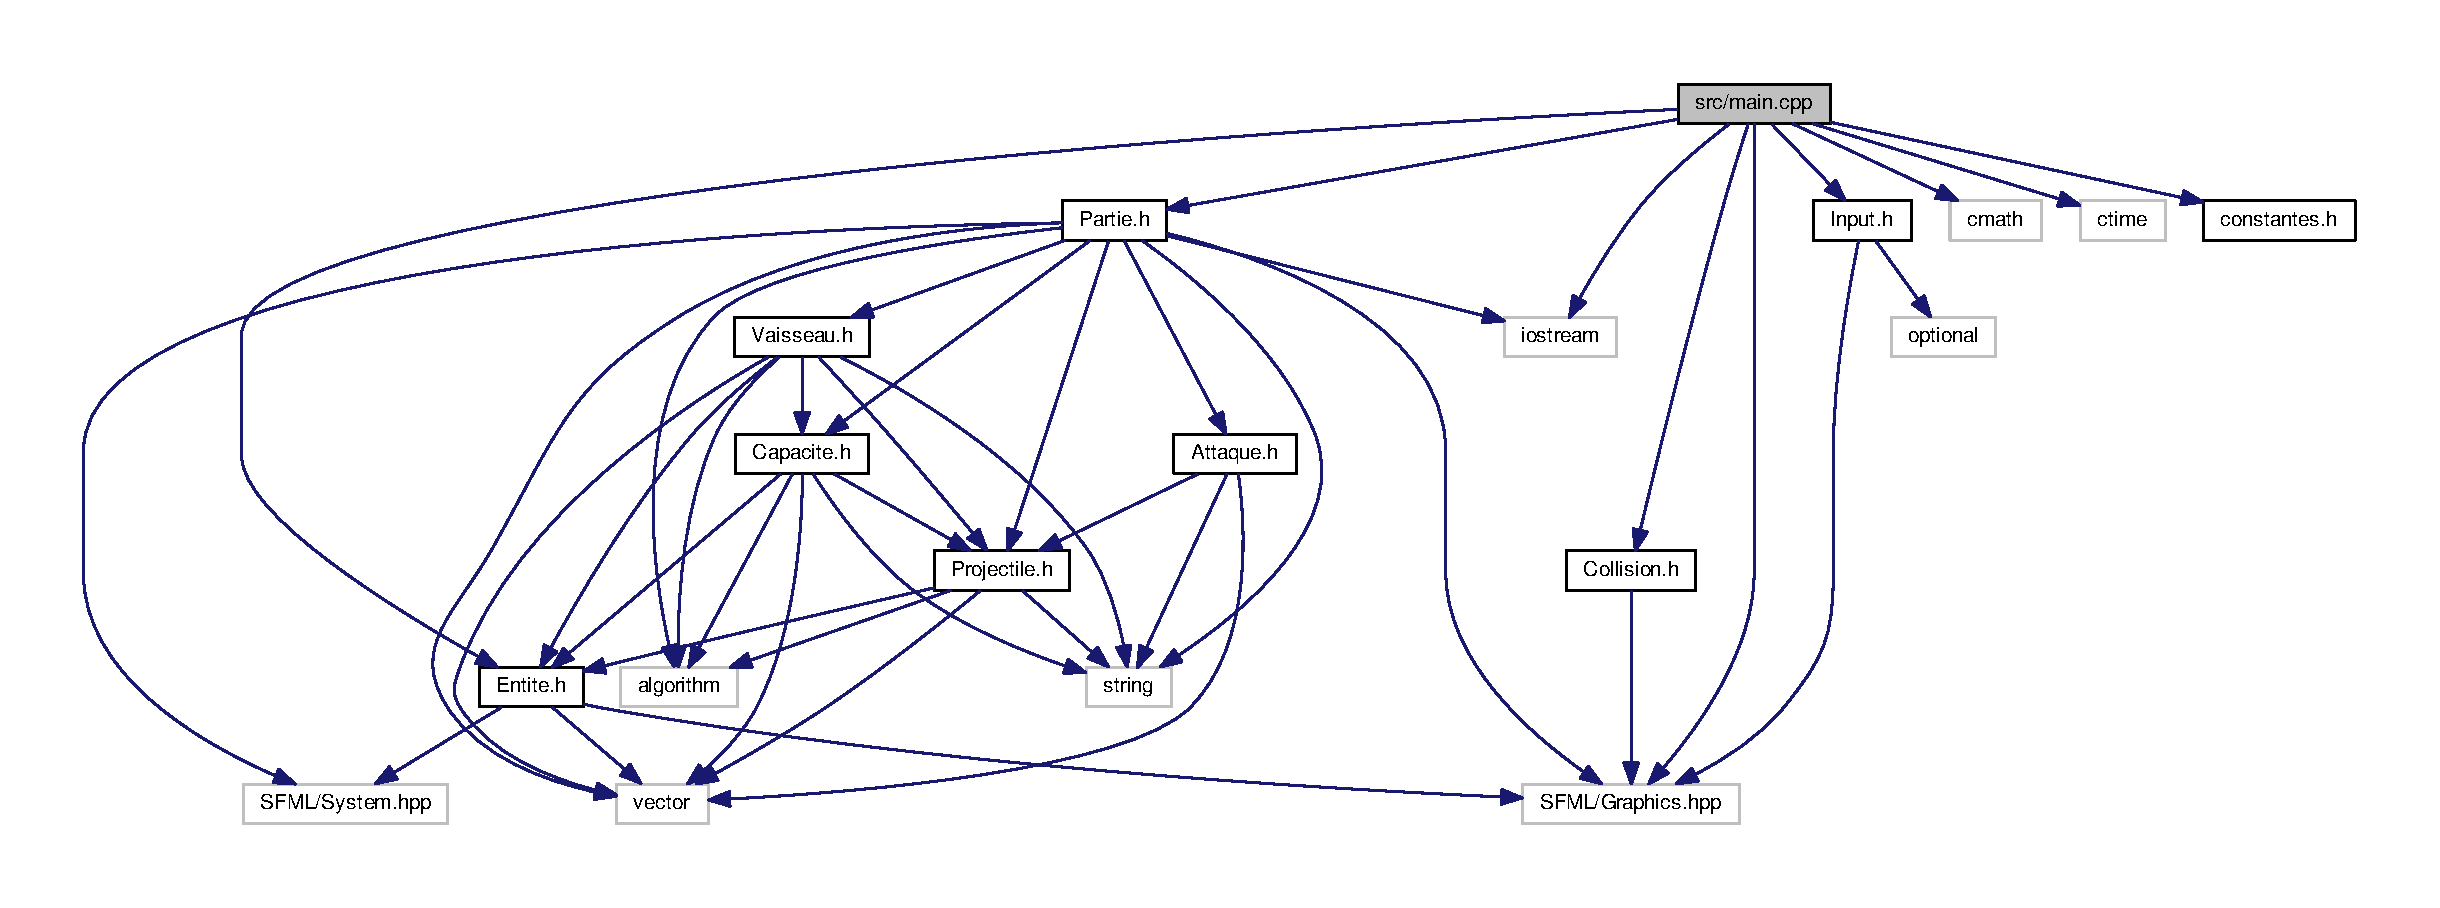
\includegraphics[width=350pt]{main_8cpp__incl}
\end{center}
\end{figure}
\subsection*{Fonctions}
\begin{DoxyCompactItemize}
\item 
int \hyperlink{main_8cpp_ae66f6b31b5ad750f1fe042a706a4e3d4}{main} ()
\end{DoxyCompactItemize}


\subsection{Documentation des fonctions}
\mbox{\Hypertarget{main_8cpp_ae66f6b31b5ad750f1fe042a706a4e3d4}\label{main_8cpp_ae66f6b31b5ad750f1fe042a706a4e3d4}} 
\index{main.\+cpp@{main.\+cpp}!main@{main}}
\index{main@{main}!main.\+cpp@{main.\+cpp}}
\subsubsection{\texorpdfstring{main()}{main()}}
{\footnotesize\ttfamily int main (\begin{DoxyParamCaption}{ }\end{DoxyParamCaption})}

$<$attention très bordélique 
\hypertarget{_partie_8h}{}\section{src/\+Menu/\+Partie.h File Reference}
\label{_partie_8h}\index{src/\+Menu/\+Partie.\+h@{src/\+Menu/\+Partie.\+h}}
{\ttfamily \#include $<$vector$>$}\newline
{\ttfamily \#include $<$string$>$}\newline
{\ttfamily \#include $<$algorithm$>$}\newline
{\ttfamily \#include $<$iostream$>$}\newline
{\ttfamily \#include $<$memory$>$}\newline
{\ttfamily \#include $<$S\+F\+M\+L/\+Graphics.\+hpp$>$}\newline
{\ttfamily \#include $<$S\+F\+M\+L/\+System.\+hpp$>$}\newline
{\ttfamily \#include \char`\"{}../\+Capacites/\+Capacite.\+h\char`\"{}}\newline
{\ttfamily \#include \char`\"{}../\+Projectiles/\+Projectile.\+h\char`\"{}}\newline
{\ttfamily \#include \char`\"{}../\+Vaisseau/\+Vaisseau.\+h\char`\"{}}\newline
{\ttfamily \#include \char`\"{}../\+Interface/\+Input.\+h\char`\"{}}\newline
{\ttfamily \#include \char`\"{}../\+Interface/\+Overlay.\+h\char`\"{}}\newline
{\ttfamily \#include \char`\"{}../\+Pattern/\+Vague.\+h\char`\"{}}\newline
{\ttfamily \#include \char`\"{}../def\+\_\+type.\+h\char`\"{}}\newline
{\ttfamily \#include \char`\"{}Ecran.\+h\char`\"{}}\newline
\subsection*{Classes}
\begin{DoxyCompactItemize}
\item 
class \mbox{\hyperlink{class_partie}{Partie}}
\begin{DoxyCompactList}\small\item\em Description brève. \end{DoxyCompactList}\end{DoxyCompactItemize}

\hypertarget{_projectile_8h}{}\section{Référence du fichier src/\+Projectiles/\+Projectile.h}
\label{_projectile_8h}\index{src/\+Projectiles/\+Projectile.\+h@{src/\+Projectiles/\+Projectile.\+h}}
{\ttfamily \#include $<$vector$>$}\newline
{\ttfamily \#include $<$string$>$}\newline
{\ttfamily \#include $<$algorithm$>$}\newline
{\ttfamily \#include \char`\"{}../\+Entite.\+h\char`\"{}}\newline
Graphe des dépendances par inclusion de Projectile.\+h\+:\nopagebreak
\begin{figure}[H]
\begin{center}
\leavevmode
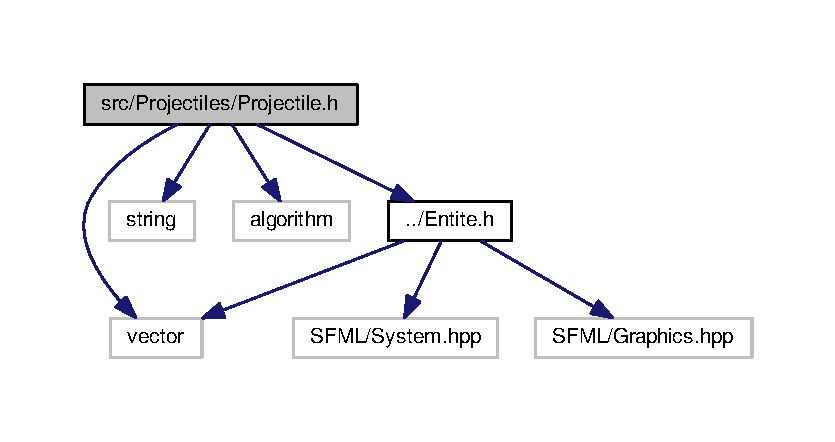
\includegraphics[width=350pt]{_projectile_8h__incl}
\end{center}
\end{figure}
Ce graphe montre quels fichiers incluent directement ou indirectement ce fichier \+:\nopagebreak
\begin{figure}[H]
\begin{center}
\leavevmode
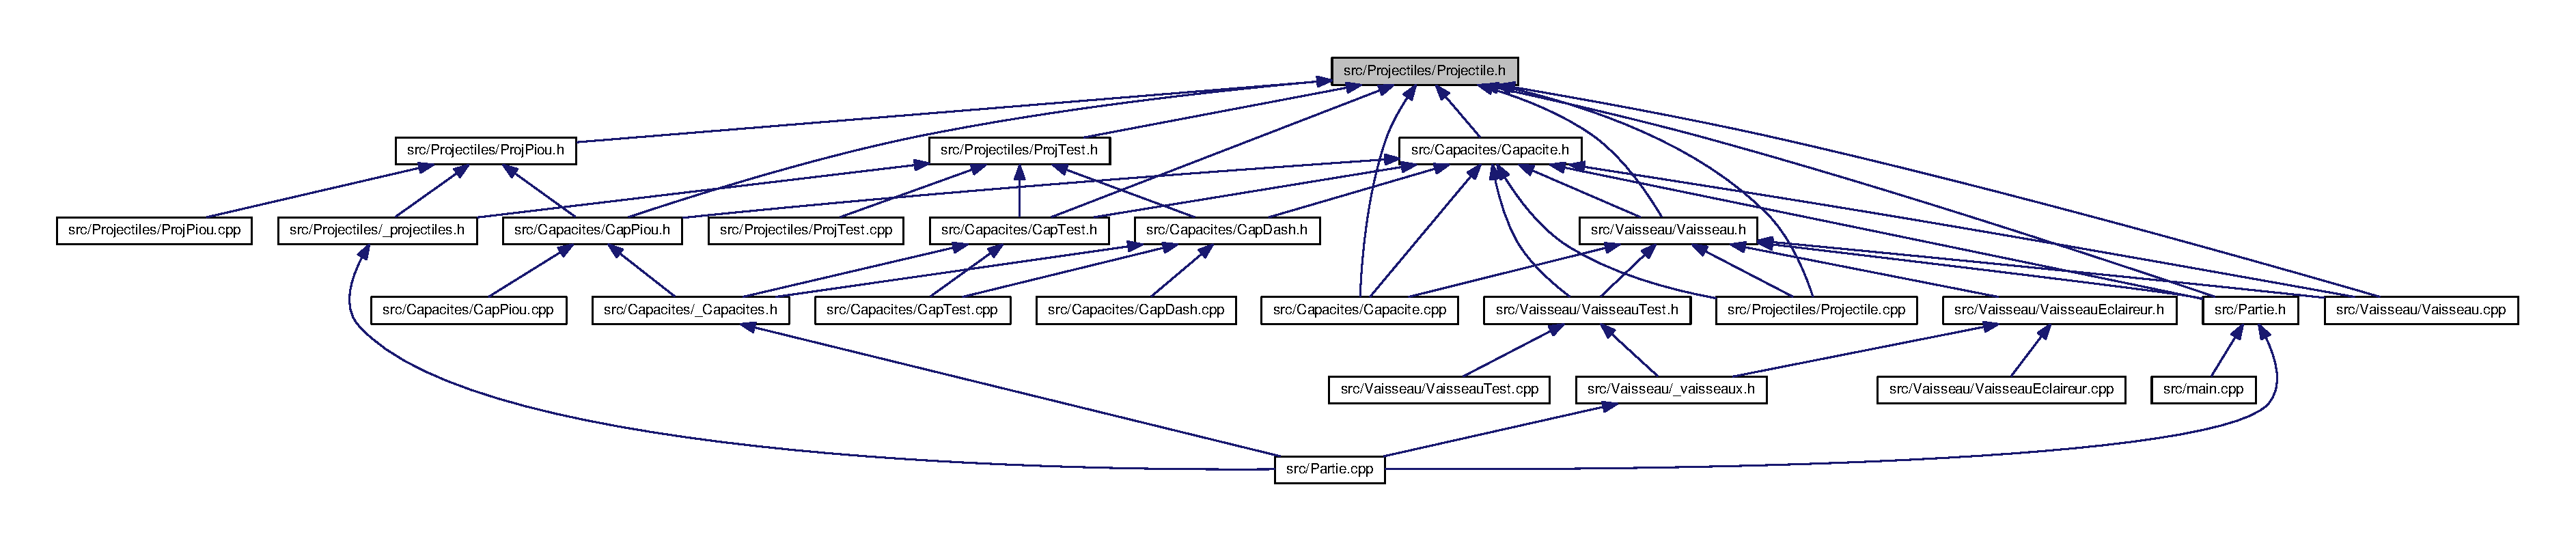
\includegraphics[width=350pt]{_projectile_8h__dep__incl}
\end{center}
\end{figure}
\subsection*{Classes}
\begin{DoxyCompactItemize}
\item 
class \hyperlink{class_projectile}{Projectile}
\begin{DoxyCompactList}\small\item\em Classe abstraite qui définit la structure générale d\textquotesingle{}un projectile, à faire hériter pour chaque projectile. \end{DoxyCompactList}\end{DoxyCompactItemize}

\hypertarget{_vaisseau_8h}{}\section{Référence du fichier src/\+Vaisseau/\+Vaisseau.h}
\label{_vaisseau_8h}\index{src/\+Vaisseau/\+Vaisseau.\+h@{src/\+Vaisseau/\+Vaisseau.\+h}}
{\ttfamily \#include $<$vector$>$}\newline
{\ttfamily \#include $<$string$>$}\newline
{\ttfamily \#include $<$algorithm$>$}\newline
{\ttfamily \#include \char`\"{}../\+Capacites/\+Capacite.\+h\char`\"{}}\newline
{\ttfamily \#include \char`\"{}../\+Entite.\+h\char`\"{}}\newline
{\ttfamily \#include \char`\"{}../\+Projectiles/\+Projectile.\+h\char`\"{}}\newline
Graphe des dépendances par inclusion de Vaisseau.\+h\+:\nopagebreak
\begin{figure}[H]
\begin{center}
\leavevmode
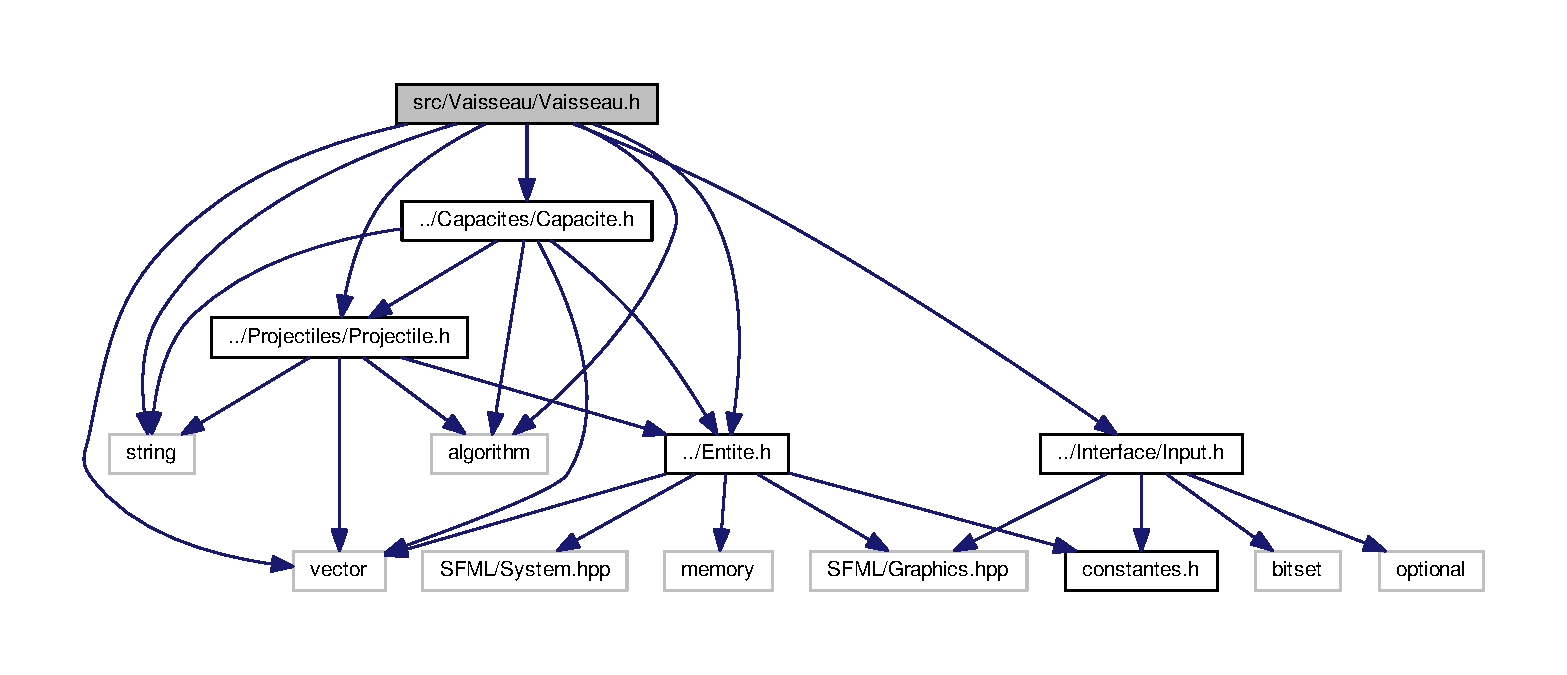
\includegraphics[width=350pt]{_vaisseau_8h__incl}
\end{center}
\end{figure}
Ce graphe montre quels fichiers incluent directement ou indirectement ce fichier \+:\nopagebreak
\begin{figure}[H]
\begin{center}
\leavevmode
\includegraphics[width=350pt]{_vaisseau_8h__dep__incl}
\end{center}
\end{figure}
\subsection*{Classes}
\begin{DoxyCompactItemize}
\item 
class \hyperlink{class_vaisseau}{Vaisseau}
\begin{DoxyCompactList}\small\item\em classe du vaisseau (véhicule) d\textquotesingle{}un joueur ou d\textquotesingle{}un ennemi \end{DoxyCompactList}\end{DoxyCompactItemize}

%--- End generated contents ---

% Index
\backmatter
\newpage
\phantomsection
\clearemptydoublepage
\addcontentsline{toc}{chapter}{Index}
\printindex

\end{document}
